\documentclass[secnumaric,notitlepage,amsmath,amssymb,nofootinbib,floatfix,12pt]{revtex4-1}
%\documentclass[12pt]{article}
\usepackage{amsfonts}
\usepackage{amssymb}
\usepackage{amsmath}
\usepackage{color}
\usepackage{graphicx}
\usepackage{enumitem}
\usepackage{algorithm}
\usepackage{algpseudocode}

\DeclareMathOperator*{\argmax}{arg\,max}
\DeclareMathOperator*{\argmin}{arg\,min}

%%%%%%%%%%%%%%%%%%%%%%%%%%%%%%%%%%%%%%%%%%%%%%%%%%%%%%%%%%%
\begin{document}
\title{6.437 Project Part I}
\author{Robert Arnott}
\date{\today}

\maketitle
%%%%%%%%%%%%%%%%%%%%%%%%%%%%%%%%%%%%%%%%%%%%%%%%%%%%%%%%%%%
\section*{Problem 1: Framework}
\begin{enumerate}[label=(\alph*)]
\item 
\begin{equation}
p_{\mathbf{y}|f}(\mathbf{y}|f) = p_{\mathbf{x}}(\mathbf{x} = f^{-1}(\mathbf{y})) = p_{\mathbf{x}}(f^{-1}(y_1)) \prod_{i=1}^{n-1} p_{x|x}(f^{-1}(y_{i+1})|f^{-1}(y_{i}))
\end{equation}
\item Using $p_{\mathbf{y}|f}(\mathbf{y}|f)$ as specified in part (a), we can find $p_{f|\mathbf{y}}(f|\mathbf{y})$:
\begin{equation}
\begin{split}
p_{f|\mathbf{y}}(f|\mathbf{y}) &= \frac{p_{\mathbf{y}|f}(\mathbf{y}|f)p_f(f)}{\sum_{f \in \mathcal{F}} p_{\mathbf{y}|f}(\mathbf{y}|f)p_f(f)} \\
&= \frac{p_{\mathbf{y}|f}(\mathbf{y}|f)(\frac{1}{m!})}{\sum_{f \in \mathcal{F}} p_{\mathbf{y}|f}(\mathbf{y}|f)(\frac{1}{m!})} \\
&= \frac{p_{\mathbf{y}|f}(\mathbf{y}|f)}{\sum_{f \in \mathcal{F}} p_{\mathbf{y}|f}(\mathbf{y}|f)}
\end{split}
\end{equation}
Where $\mathcal{F}$ is the family of all permutations $f$ on the alphabet $\mathcal{A}$, so that $|\mathcal{F}| = (|\mathcal{A}|)! = m!$ and where we have use that $f$ is drawn uniformly at random from $\mathcal{F}$.\par
This gives that the MAP estimator $\hat{f}_{MAP} = \argmax_{f\in \mathcal{F}} p_{f|\mathbf{y}}(f|\mathbf{y})$ is $\hat{f}_{MAP} = \argmax_{f\in \mathcal{F}} p_{\mathbf{y}|f}(\mathbf{y}|f)$, which we note, implies $\hat{f}_{MAP} = \hat{f}_{MLE}$
\item Direct computation of $f_{MAP}$ is infeasible as computing the normalization factor requires calculating $p_{\mathbf{y}|f}(\mathbf{y}|f)$ $m!$ times (for each possible $f$). In addition, for any decently long sequence, $p_{\mathbf{y}|f}(\mathbf{y}|f)$ is essentially $0$.
\end{enumerate}

%%%%%%%%%%%%%%%%%%%%%%%%%%%%%%%%%%%%%%%%%%%%%%%%%%%%%%%%%%%
\section*{Problem 2: Markov Chain Monte Carlo Method}
\begin{enumerate}[label=(\alph*)]
\item There are $\binom{m}{2}$ ways to pick the difference, and $m!$ possible choices for $f_1$. Further, choosing $f_1$ fixes $f_2$, since there is only one way for the two assignments to differ (swap them). Thus, since there $(m!)^2$ total possible choices for $f_1,f_2$, the probability that $f_1$ and $f_2$ differ by exactly two assignments is $\frac{\binom{m}{2}}{m!}$
\item Let the set $S(f_i) = \{ f_j \, | \, \text{$f_j$ differs from $f_i$ by exactly 2 assignments} \}$. We can use the proposal:
\[ V(f^{\prime} | f) = 
\begin{cases} 
      \frac{\epsilon}{\binom{m}{2}} & f^{\prime} \in S(f) \\
      1-\epsilon & f^{\prime}=f \\
      0 & \text{otherwise} 
   \end{cases}
\] (i.e. with probability $\epsilon$, $V$ is uniform over the set of permutation functions that differ by exactly two assignments, otherwise, $V$ picks $f^{\prime}=f$). Here, $\epsilon \in (0,1)$ is a model parameter. Note that this proposal is symmetric between $f^{\prime}$ and $f$. \par
Under this proposal, the generated Markov Chain is irreducible (we can reach any $f\in\mathcal{F}$ from some $f_0 \in \mathcal{F}$, by continuing to change two assignments at a time), and the Markov chain is aperiodic (since each state can transition back to itself, with guaranteed non-zero probability). This ensures that the Markov Chain has a stationary distribution (i.e. is homogeneous), and thus by results given in lecture notes, that stationary distribution is $p_{f|\mathbf{y}}(f|\mathbf{y})$
\item We use the following algorithm to find a decoder:
\begin{algorithmic}
\State Initialize $f_0$ as a random draw from $\mathcal{F}$
\Repeat \;{On iteration $n$}
	\State Generate sample $f^{\prime}$ from $V(\cdot | f_n)$
	\State Compute $a = \min (1, \frac{p_{\mathbf{y}|f^{\prime}}(\mathbf{y}|f^{\prime})}{p_{\mathbf{y}|f}(\mathbf{y}|f_n)})$
	\State Generate sample $u$ from $\mathcal{U}([0,1])$ (uniform distribution)
	\If {$u \leq a$}
		\State Accept the proposed sample, and set $f_{n+1} = f^{\prime}$
	\Else
		\State Reject the proposed sample, and set $f_{n+1} = f_n$
	\EndIf
\Until {Desired number of iterations or convergence}
\State Find the generated estimate $\hat{f}_{MAP} = \argmax_{f \in \mathcal{F}_N} p_{\mathbf{y}|f}(\mathbf{y}|f)$, where $\mathcal{F}_n$ is the set of samples generated during the iterations, potentially after discarding some set of initial samples to account for "burn-in"
\end{algorithmic}
\end{enumerate}

%%%%%%%%%%%%%%%%%%%%%%%%%%%%%%%%%%%%%%%%%%%%%%%%%%%%%%%%%%%
\section*{Problem 3: Implementation}
\begin{enumerate}[label=(\alph*)]
\item We obtain the behavior shown in Figure ~\ref{fig:log-likelihood}.
\begin{figure}[htb]
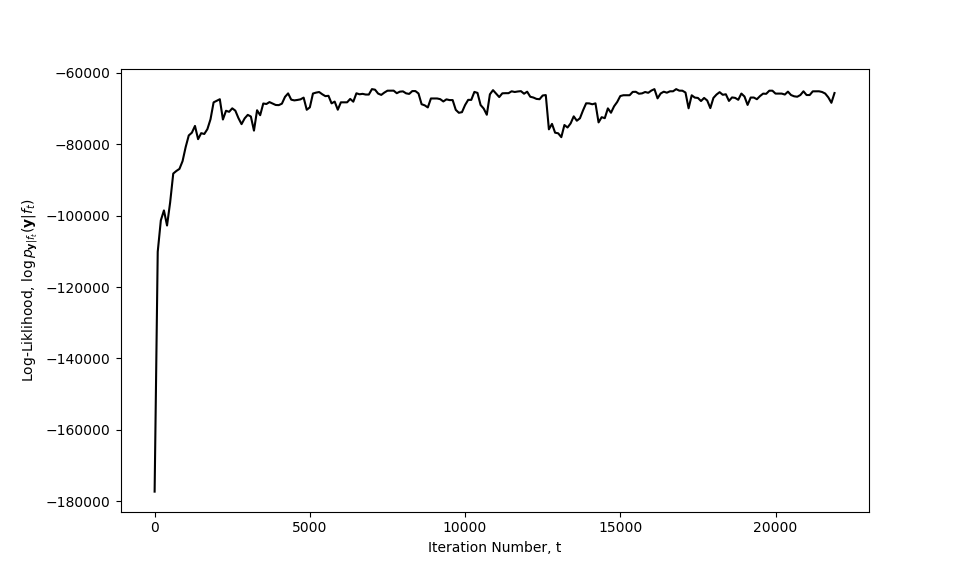
\includegraphics[scale=0.7]{../plots/log-likelihood_vs_iteration.png}
\caption{The evolution of the log-likelihood $\log p_{\mathbf{y}|f}(\mathbf{y}|f_t)$ over the course of the run. Burn-in samples are included.}
\label{fig:log-likelihood}
\end{figure}
\item We obtain the behavior shown in Figure ~\ref{fig:acceptance-rates}.
\begin{figure}
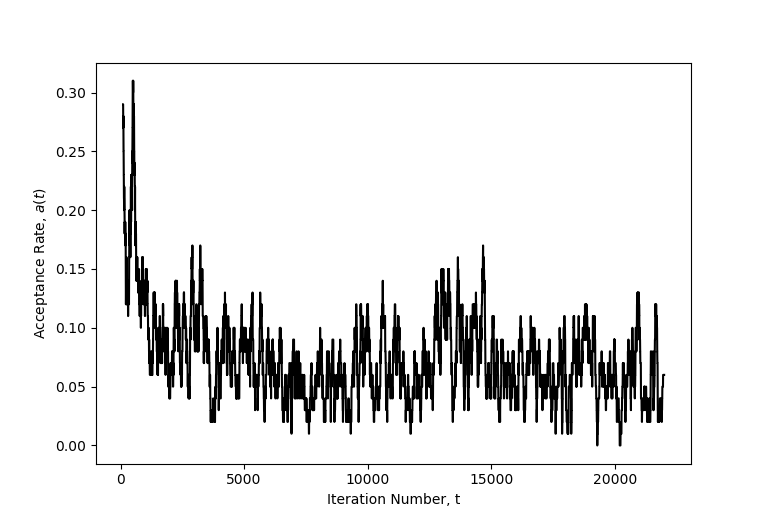
\includegraphics[scale=0.7]{../plots/acceptance_rate.png}
\caption{The evolution of the acceptance rate $a(t)$ over the course of the run, calculated over a sliding window of 200 iterations. Burn-in samples are included.}
\label{fig:acceptance-rates}
\end{figure}
\item We obtain the behavior shown in Figure ~\ref{fig:accuracies}.
\begin{figure}[htb]
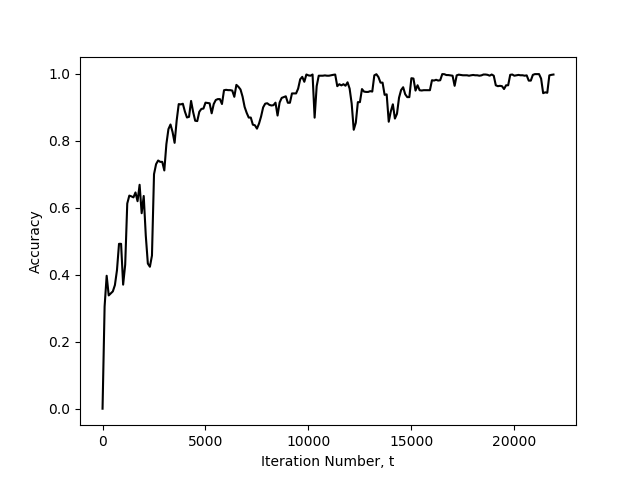
\includegraphics[scale=0.7]{../plots/accuracy_vs_iteration.png}
\caption{The evolution of the accuracy $\beta(t)$ over the course of the run. Burn-in samples are included.}
\label{fig:accuracies}
\end{figure}
\item We note that in general, the longer the sequence we allow our algorithm to run on, the higher the observed accuracy. This is intuitively true as we have that longer sequences will tend to behave more like the true distribution of the alphabet, and thus make it easier to separate out different permutation functions. This is shown in the empirical results shown in Figure ~\ref{fig:accuracy-vs-length}.
\begin{figure}[htb]
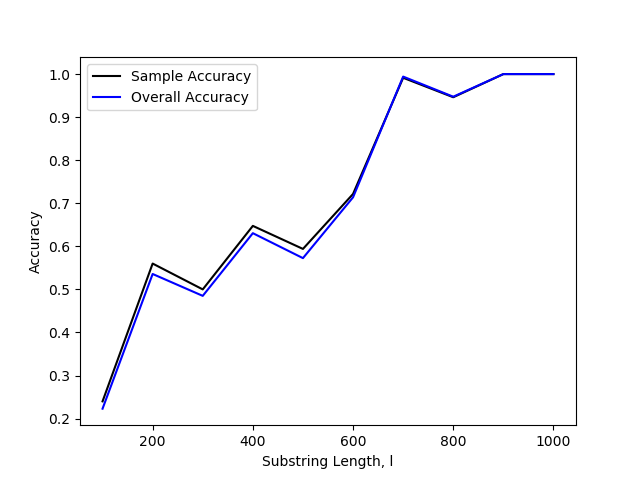
\includegraphics[scale=0.6]{../plots/accuracy_vs_length.png}
\caption{The relationship between the accuracy $\beta(t)$ and the length of the sub-sequence of the ciphertext seen by the algorithm. Accuracy is measured both with respect to the sub-sequence given to the algorithm (``Sample Accuracy") and with regards to the entire ciphertext (``Overall Accuracy")}
\label{fig:accuracy-vs-length}
\end{figure}
\item We obtain the behaviour shown in Figure ~\ref{fig:per-char-ll}. We note that the per character log-likelihood converges to a value slightly larger than the negative of the entropy of the letter distribution.
\begin{figure}[htb]
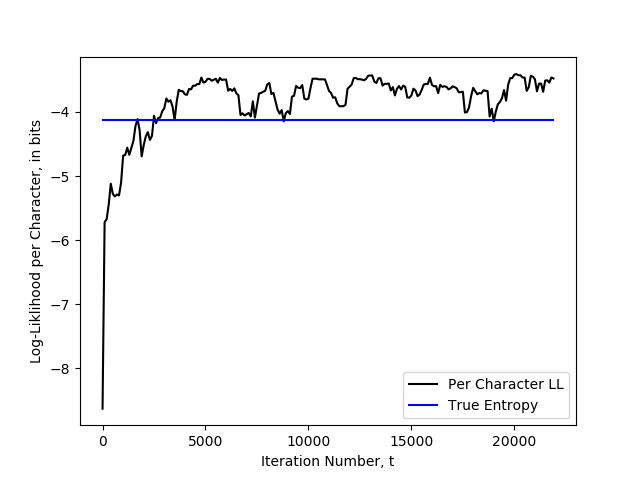
\includegraphics[scale=0.6]{../plots/per_character_log-likelihood_vs_iteration.png}
\caption{The evolution of the per character log-likelihood $\frac{1}{N} \log_2 p_{\mathbf{y}|f}(\mathbf{y}|f_t)$ (measured in bits) over the course of the run, plotted alongside the negative of the entropy of the given letter distribution. Burn-in samples are included.}
\label{fig:per-char-ll}
\end{figure}
\end{enumerate}
\end{document}